%------------------- Limbs -------------------%
\subsection{Limbs} \label{subsec:limbs}
The robot is composed of five legs, all of which are identical in size and length. For this reason, only one leg is analyzed when subject to worst case scenario forces. However, as the robot configuration is not symmetrical for the frontal legs and rear legs, some legs will never be submitted to worst case scenario forces.
\subsubsection{Inputs and Outputs}
 The inputs are the links length determined by optimal link length analysis, the size of internal component such as the pulley at the knee, and the normal and friction force found at the foot. 
 This analysis does not output any parameters to other components analysis. This analysis ensures a reasonable safety factor and determines the diameter and thickness of the tibia, where possible.   

\subsubsection{Constants and Parameters}
The lengths, angle and sizes of the limbs must be known to calculate the bending and shearing in the limbs. They are predetermined by optimal limb length analysis which establishes the legs reach and height. Some limitations exist such as the size of the pulley which restricts the minimal size of the thigh member. The normal force and friction force are found using external force analysis. For this analysis, the worst case scenario of both frictional forces and normal forces are used. The circular tube thickness is set constant at 1.6 mm due to industry standards. The targeted safety factor for this section is 2.0 due to unknown external forces such as human interactions, obstacles, drops, etc. 

\subsubsection{Assumptions and Simplifications}
Limb weight were assumed as they cannot be calculated until the size the limbs are determined by this analysis which creates an iterative process. The weight of the foot is included in the weight of member 3 ($m_3$) and the weight of the knee is included in the weight of member 2 ($m_2$) as shown in Figure \ref{fig:fbd_leg}. The weights have been assumed to be in the centre of the member whereas the weight should technically be distributed over the whole member. In between point B and C, the member is press fitted to a mounting piece, no calculation on the press fit was performed as it was assumed a non critical failure location due to only compression forces and relatively small bending forces.

\subsubsection{Material Selection}
The material selected for the application of the limb is marine grade aluminum 6061-T6 for its outdoor resistance, high yield strength of about 276 MPa and low mass \cite{matweb_aluminum_nodate}.

\subsubsection{Free-Body Diagram}
First, the FBD of the leg is used to determine external forces on the members. This is shown in Figure \ref{fig:fbd_leg}. External forces are the frictional forces $F_f$ and reactive forces perpendicular to the ground $F_N$. A friction force at the foot in the y direction is not shown in the FBD but included in the calculation.
\begin{figure}
    \centering
    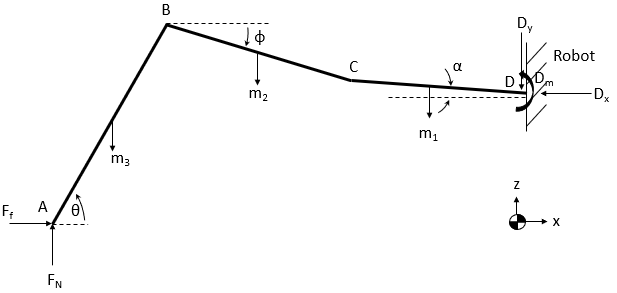
\includegraphics[width=\textwidth]{4_Analysis/img/Limbs/Leg_FBD.PNG}
    \caption{Force-Body Diagram of one leg}
    \label{fig:fbd_leg}
\end{figure}

To properly analyse all members/links of the leg, the leg must be decomposed into its various sections. The leg is decomposed into three sections, AB which is the foot and lower tibia, BC is the higher tibia, and CD is the thigh. The decomposition enables to calculate internal forces at the joint of all members as shown in Figure \ref{fig:fbd_leg_section} where $r_3$, $r_2$, $r_1$ are length of the member, $B_m$, $C_m$, and $D_m$ are moments at the joints and all other arrow are forces.

\begin{figure}
    \centering
    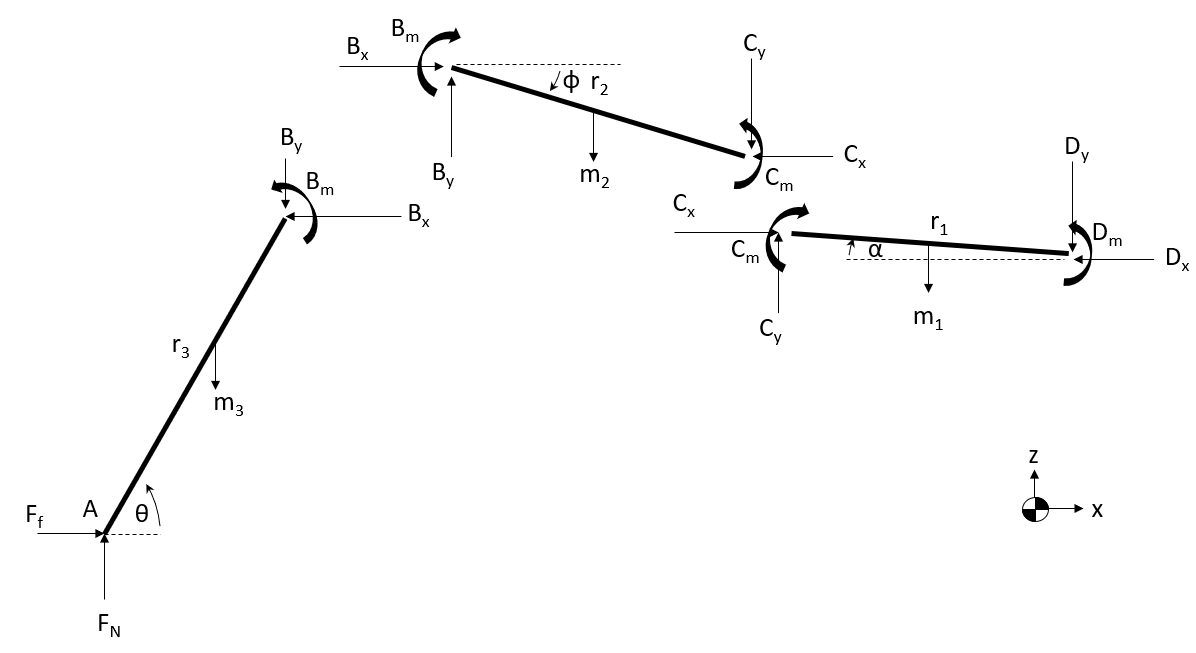
\includegraphics[width=\textwidth]{4_Analysis/img/Limbs/Leg_Decomposed.PNG}
    \caption{Force-Body Diagram for inner forces}
    \label{fig:fbd_leg_section}
\end{figure}
\subsubsection{Stress Analysis}
To calculate the stress in the members, first the axial, radial and bending forces must be determined. Using the sum of forces and moments about an axis, the joint forces $B_{x,y}$, $C_{x,y}$ and $D_{x,y}$, and moments $B_M$, $C_M$, $D_M$ can be determined as follows.

\begin{equation}
\sum F_{x_{AB}} = 0 = F_f - B_x \rightarrow B_x = F_f = 10.6N
\end{equation}

\begin{equation}
\begin{split}
        \sum &F_{y_{AB}} = 0 = F_N - m_3 g -B_y \rightarrow
        \\
        &B_y = F_N - m_3 g = 160N-(0.532kg)(9.81m/s^2) = 154.8N
    \end{split}
\end{equation}

\begin{equation}
\sum F_{x_{BC}} = 0 = B_x - C_x \rightarrow C_x = B_x = 10.6N
\end{equation}

\begin{equation}
\begin{split}
        \sum &F_{y_{BC}} = 0 = B_y - m_2 g -C_y \rightarrow 
        \\
        &C_y = B_y - m_2 g = 154.8N - (0.836 kg)(9.81m/s^2) = 146.6N
    \end{split}
\end{equation}

\begin{equation}
\sum F_{x_{CD}} = 0 = C_x - D_x \rightarrow D_x = C_x = 10.6N
\end{equation}

\begin{equation}
    \begin{split}
        \sum &F_{y_{CD}} = 0 = C_y - m_1 g -D_y \rightarrow 
        \\ 
        &D_y = C_y - m_1 g = 146.6N - (0.532kg)(9.81m/s^2) = 141.4N
    \end{split}
\end{equation}
    
    \begin{gather}
    \begin{split}
    \sum M_B &= 0 = -F_N r_3 \sin{\theta} + F_f r_3 \cos{\theta} + m_3 g \frac{r_3}{2} \cos{\theta} + B_M  \rightarrow
    \\
    B_M &= F_N r_3 \sin{\theta} - F_f r_3 \cos{\theta} - m_3 g\frac{r_3}{2} \cos{\theta}
    \\
    B_M &= (160N)(300mm) \sin{(71.3 deg)} - (10.6N)(300mm) \cos{(71.3 deg)} -
    \\
    &(0.532kg)(9.81m/s^2)\frac{(300mm)}{2} \cos{(71.3 deg)}
    \\
    B_M&= 12153.4Nmm
    \end{split}  \label{eq:limb_B_M}
    \end{gather}
    \begin{gather}
    \begin{split}
    \sum M_C &= 0 = -B_x r_2 \sin{\phi}- B_y r_2 \cos{\phi} + m_2 g \frac{r_2}{2}\cos{\phi} - B_M + C_M \rightarrow
        \\
     C_M &= B_x r_2 \sin{\phi}+ B_y r_2 \cos{\phi} -m_2 g \frac{r_2}{2}\cos{\phi} + B_M
     \\
    C_M &= (10.6N)(100mm) \sin{(39.8 deg)}+ (154.8N) (100mm) \cos{(39.8deg)} -
    \\
    &(0.836kg)(9.81m/s^2) \frac{(100mm)}{2}\cos{(39.8 deg)} + 12153.4Nmm 
    \\
    C_M &= 24418.6Nmm
     \label{eq:limb_C_M}
    \end{split}
    \end{gather}
    
    \begin{gather}
    \begin{split}
        \sum M_D &= 0 = -C_x r_1 \sin{\alpha} -C_y r_1 \cos{\alpha} + m_1 g \frac{r_1}{2}\cos{\alpha} - C_M +D_M \rightarrow
    \\
    D_M &= C_x r_1 \sin{\alpha} +C_y r_1 \cos{\alpha} - m_1 g \frac{r_1}{2}\cos{\alpha} +C_M 
    \\
    D_M &= (10.6N) (100mm) \sin{(17.6 deg)} +(146.6N) (100 mm) \cos{(17.6 deg)} - 
    \\
    &(0.5kg) (9.81m/s^2) \frac{(100 mm)}{2}\cos{(17.6 deg)} +24418.6 Nmm
    \\
    D_M&= 38479.1\label{eq:limb_D_M}
    \end{split}
\end{gather}

Using the internal forces convention, the axial, shear and bending forces at every point on a member/link is found using the following equations and shown in Figure \ref{fig:limb_diagram}.

Section AB:
\begin{gather}
    \text{Axial : }-F_f \cos{\theta} -F_N \sin{\theta}
    \qquad\text{Axial : }-F_f \cos{\theta} -F_N \sin{\theta} + m_3 g\sin{\theta} \label{eq:limb_AB_axial}
    \\
    \text{Radial : }-F_f \sin{\theta} + F_N \cos{\theta}
    \qquad\text{Radial : }-F_f \sin{\theta} + F_N \cos{\theta}- m_3 g \cos{\theta}\label{eq:limb_AB_radial}
\end{gather}

Section BC:
\begin{gather}
    \text{Axial : } -B_x \cos{\phi} + B_y \sin{\phi}
    \qquad\text{Axial : } -B_x \cos{\phi} + B_y \sin{\phi} - m_2 g \cos{\phi} \label{eq:limb_BC_axial}
    \\
    \text{Radial : }  B_x \sin{\phi} + B_y \cos{\phi}
    \qquad\text{Radial : }  B_x \sin{\phi} + B_y \cos{\phi}- m_2 g \sin{\phi}\label{eq:limb_BC_radial}
\end{gather}

Section CD:
\begin{gather}
    \text{Axial : } -C_x \cos{\alpha} + C_y \sin{\alpha}
    \qquad\text{Axial : } -C_x \cos{\alpha} + C_y \sin{\alpha}- m_1 g \cos{\alpha}\label{eq:limb_CD_axial}
    \\
    \text{Radial : }  C_x \sin{\alpha} + C_y \cos{\alpha}
    \qquad\text{Radial : }  C_x \sin{\alpha} + C_y \cos{\alpha}- m_1 g \sin{\alpha} \label{eq:limb_CD_radial}
\end{gather}

\begin{figure}
    \centering
    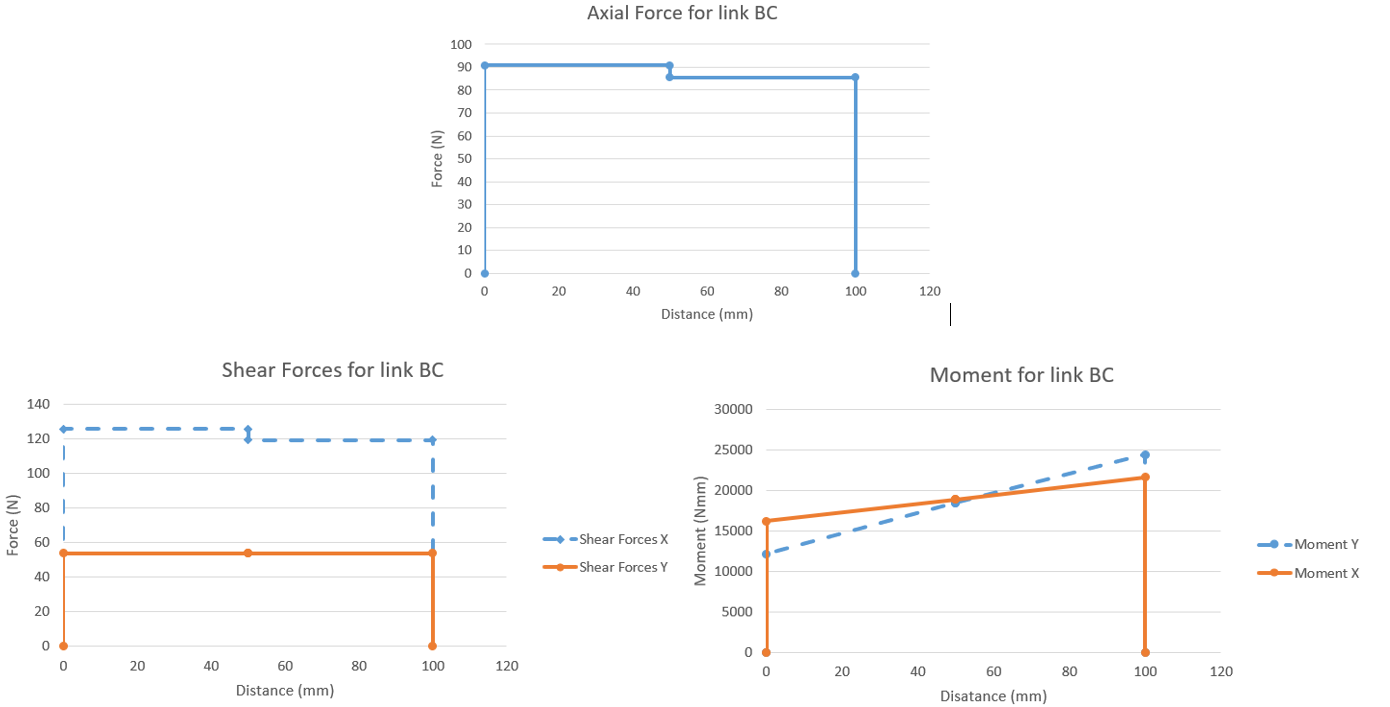
\includegraphics[width=\textwidth]{4_Analysis/img/Limbs/Forces.PNG}
    \caption{Axial Force Diagram}
    \label{fig:limb_diagram}
\end{figure}

As there are bending and shearing in multiple planes, the resultants of both are calculated as shown in equation \ref{eq:limb_V} and \ref{eq:limb_M}. The numerical values are for point C which is located at 100mm in the stress diagrams shown in Figure \ref{fig:limb_diagram}. For other members, see Appendix \ref{app:limb_analysis}.
\begin{gather}
    V = \sqrt{V_x^2 + V_y^2} = \sqrt{(119.5 N)^2 + (54.0 N)^2} = 131.1 N \label{eq:limb_V}
    \\
    M = \sqrt{M_x^2 + M_y^2} = \sqrt{(12153.4 Nmm)^2 + (16204.5 Nmm)^2} = 20255.6 Nmm \label{eq:limb_M}
\end{gather}

The bending can be obtained by multiplying the radial force to the distance such as $ \text{Bending} = \text{Radial} \times \text{Distance} $ and can then be matched to joint values such as $B_M$, $C_M$, and $D_M$ to confirm the calculations.
The bending and shear diagrams demonstrate that between both hollow circular member AB and BC, point C will have the highest stress concentration. First the axial stress is calculate using the following equation \cite{budynas_shigleys_2015}:

\begin{equation}
\begin{split}
        \sigma_x = \frac{P_x}{A} + \frac{My}{I} =  \frac{P_x}{\frac{\pi}{4} (D^2-d^2)} + \frac{My}{\frac{\pi}{64} (D^4-d^4)} 
        \\
        = \frac{85N}{\frac{\pi}{4} ((17.175mm)^2-(14mm)^2)} + \frac{(32605Nmm)(\frac{7.175mm}{2})}{\frac{\pi}{64} ((17.175mm)^4-(14mm)^4)} = 118.5 MPa   \label{eq:limb_axial}
\end{split}
\end{equation}

The shearing stress due to radial forces in the member are calculated as shown in Equation \ref{eq:limb_shear_xy}, and the shearing forces created by the torsion due to frictional forces in the y direction (when on a slope) is shown in Equation \ref{eq:limb_torsion}.

\begin{gather}
    \tau_{shear_{xy}} = \frac{2V}{A}= \frac{2(131.1N)}{\frac{\pi}{4} ((17.175mm)^2-(14mm)^2)} = 3.37 MPa \label{eq:limb_shear_xy}
    \\
    \tau_{torsion} = \frac{T}{2r^2t} = \frac{(15128Nmm)}{2(1.59mm)(7.79mm)^2} = 24.9 MPa
    \label{eq:limb_torsion}
    \\
    \tau_{xy} = \tau_{shear_{xy}} +  \tau_{torsion}= 3.4 MPa + 24.9MPA = 28.3 MPa
\end{gather}

The safety factor $n$ of the limb to external forces is calculated by comparing the Von Mises equivalent stress $\sigma_e$ and yield strength $S_y$ of the material.
\begin{gather}
\sigma_e = (\sigma_x^2+3\tau_{xy}^2)^{(1/2)} = ((118.5 MPa)^2 + 3(28.3 MPa)^2)^{(1/2)} = 128.2 MPa  \label{eq:limb_equivalent}
\\
n = \frac{S_y}{\sigma_e} = \frac{250 MPa}{128.2 MPa} = 2.0
\end{gather}


Another critical location on the member is the curved section of the beam which is at point B. As the member is considered a curved beam, different set of equations are used. Equations for hollow circular cross sections for curved beams could not be found nor derived, thus the stress in the beam was approximated using a full tube cross section and a suggested approximation formula. The radius of the curvature, or the radius of inner fiber $r_i$ was set at 8.59 mm, half of the diameter of the bar which is possible in the industry but will mostlikely require advanced tooling \cite{listertube_tube_nodate}.  The radius of centroidal axis $r_c$, radius of neutral axis $r_n$ and the distance from centroidal axis to neutral axis $e$ are calculated as follow for a full circular tube where $R$ is the radius of the tube. 
\begin{gather}
r_c = r_i + R = 8.59mm + 8.59mm = 17.175 mm
\\
r_n = \frac{R^2}{2(r_c - \sqrt{r_c^2-R^2})} = \frac{(8.59 mm)^2}{2(17.175 mm - \sqrt{(17.18 mm)^2-(8.59 mm)^2})} =  16.02 mm
\\
e = r_c - r_n = 17.18 mm - 16.02 mm = 1.51 mm
\end{gather}

The stress in the curvature is calculated at the inner fiber radius $\sigma_i$, due to its higher tension forces than at the outer fiber. Where A is the area for the cross section of a hollow tube and not of a full tube.

\begin{gather}
\sigma_i = \frac{Mc_i}{Aer_i} = \frac{(20256 Nmm)(7.437 mm)}{\frac{\pi}{4} ((17.175mm)^2-(14mm)^2) (1.505 mm)(8.59 mm)} = 196.1 MPa  \label{eq:limb_curved_stress}
\end{gather}

The stress at the inner fiber of the tube is thus 196.13 MPa compared to the 72.92 MPa previously calculated at point B using straight beam formulas. The safety factor for the point B is 1.27 when subject to 196.1 MPa, however multiple assumptions were made such that the tube was hollow. If the area of a full tube is used in the above equation, a safety factor of 3.7 is achieved and if the simplification method is used a safety factor of 2.2 is achieved, see appendix \ref{app:approximation_curved_beam}. Due to the approximations, the low safety factor is acceptable in this case and the parametrization will ensure the safety factor at Point C is respected at 2.0.




\subsubsection{Critical Review}
Multiple assumptions such as the weight of the limbs and weight location were made to simplify the calculations. The stresses at the curved locations must be calculated using more advanced tools to properly determine a safety factor. Fatigue was not considered in this analysis due to the slow speed of the robot. Calculation of the weight of a member such as the lower tibia demonstrate a weight of 0.06 kg, one tenth of the approximated weight of the tibia of 0.5 kg with negligible impact on the overall bending and shear stress of the member. 

\subsubsection{Parameterization}
Due to exterior conditions, loads and application, marine grade metals are best used for the limbs of the robot. This material will not be parameterized and will remain constant for various sizes of robots. Due to the limitation posed by the pulley found at the knee, the thigh member's size is restricted by the belt and pulley size, and height requirements, thus the thigh size are determined by the section \ref{subsec:belt}, these sizes will produce very high safety factors. The length of members are also determined by external analysis. The diameter and thickness of the tibia hollow tube are parametrizable, however both are dependent of the other. To attain reasonable safety factors between 1 and 2.5, the thickness will be constant to ensure the thickness does reduces to unreasonable size. However, it is also possible that the diameter reduces to unfeasible sizes, thus diameter will be assumed constant for these situations. The bend radius of the curved section is another paramatrizable factor which helps reduce internal stresses.   The bend radius of the curved section is set at half of the diameter of the tube, however it was found that there is limited space on the upper tibia link causing obstruction issues between the bellow mounting piece and the tibia link, and an appropriate length size issue for the press fit of the tibia. Thus, the bend radius will be set at half of the diameter when possible, but may require to be reduced furthermore due to obstructions. 
